\documentclass[11 pt]{article}

\setlength{\oddsidemargin}{-.45in}
%\setlength{\evensidemargin}{-.5in}
\setlength{\textwidth}{7.25in}
\setlength{\topmargin}{-0.95in}
\setlength{\textheight}{10.2in}

\usepackage{graphics}
\usepackage{latexsym}
\usepackage{amsfonts}
\usepackage{amsmath}
\usepackage{amsthm}
\usepackage{epstopdf}
%\usepackage{multicol}
%\usepackage{wrapfig}
\pagestyle{empty}

\usepackage[T1]{fontenc}
\usepackage{baskervald}
\usepackage[bigdelims,vvarbb]{newtxmath} 

\newcommand{\ds}{\ensuremath{\displaystyle}}
\newcommand{\tr}{\vspace{0.5in}}
\newcommand{\lr}{\vspace{1.0in}}
\newcommand{\mr}{\vspace{2.0in}}
\newcommand{\br}{\vspace{3.0in}}

\newcommand{\ps}{Problem Set~}
\newcommand{\vi}{\ensuremath{\mathbf{i}}}
\newcommand{\vj}{\ensuremath{\mathbf{j}}}
\newcommand{\vk}{\ensuremath{\mathbf{k}}}
\newcommand{\vr}{\ensuremath{\mathbf{r}}}
\newcommand{\vecv}{\ensuremath{\mathbf{v}}}
\newcommand{\vu}{\ensuremath{\mathbf{u}}}
\newcommand{\va}{\ensuremath{\mathbf{a}}}
\newcommand{\vs}{\ensuremath{\mathbf{s}}}
\newcommand{\ve}{\ensuremath{\mathbf{e}}}
\newcommand{\vx}{\ensuremath{\mathbf{x}}}
\newcommand{\vc}{\ensuremath{\mathbf{c}}}
\newcommand{\vb}{\ensuremath{\mathbf{b}}}

\usepackage{hyperref} 
\hypersetup{colorlinks=true, linkcolor=blue,  anchorcolor=blue,  
citecolor=blue, filecolor=blue, menucolor=blue, pagecolor=blue,  
urlcolor=blue,pdftitle={MTH 202 Checkpoint}}

\usepackage{framed}

\newcommand{\bdr}{\ensuremath{\mathbb{R}}}

\newcommand{\be}{\begin{enumerate}}
\newcommand{\ee}{\end{enumerate}}

\newcommand{\bi}{\begin{itemize}}  
\newcommand{\ei}{\end{itemize}}

%\renewcommand{\baselinestretch}{1.5}


\begin{document}
 \hfill Boelkins \\
 
\begin{center}
Math 202-06 \\
{\bf Checkpoint 1}
\end{center}


\noindent {\bf Directions:}

\begin{itemize}
	
	\item {\bf Desmos.} You may use \href{https://www.desmos.com/calculator}{\emph{Desmos}} for computations and graphing, just like we do during class.  Any work done in \emph{Desmos} must be summarized and briefly explained in writing on your paper.  
	
	\item {\bf Resources.} During each checkpoint, you may access your own 1 page of study notes, plus \emph{Desmos}; no other uses of your computer or tablet are permitted unless specified directly.  No collaboration with other human beings or other internet resources are allowed.
	
%	\emph{Note well: if you collaborate with someone else, it is often obvious that collaboration has occurred.  Please do not put your academic standing at risk by doing this.}
	
	\item {\bf Competence.} Each week, your goal is to demonstrate competence on as many of the included learning targets as you can.  Each question will be marked either ``Y'' or ``NY'': Y for ``yes'', NY for ``not yet''.  Every learning target will appear on three different checkpoints, so you'll have multiple attempts to demonstrate your understanding.  ``Competence'' is defined as work that demonstrates clear and complete understanding of the relevant concepts in the learning target. While the work may include a minor error, or one or two minor steps may not be well explained, otherwise the work is complete, correct, and convincing, including the proper use of notation, and appropriate explanation of meaning that uses correct terminology.  (On rare occasions, you might get a ``NY*''; such a mark means you are close to competence and that you have the option to have a short conversation with me prior to the next Checkpoint and attempt to demonstrate ``Y''-level understanding through the conversation aloud.)	
\end{itemize}

\noindent \hrulefill \\

\noindent {\bf Learning Targets:} For Checkpoint \#1, there are two learning targets being assessed: 

\begin{quote}
{\bf LT 1}: I can do three key things from first semester calculus: (a) sketch the derivative function, given a function’s graph; (b) apply the chain rule to find the derivative of a composite function; and (c) apply the First Fundamental Theorem of Calculus to evaluate a definite integral. (Sections 1.4, 2.5, and 4.4)
\end{quote}

\begin{quote}
{\bf LT 2}: Given the graph of a function and other data, I can construct an accurate graph of the antiderivative of the function by determining select values of the antiderivative as well as where the antiderivative is increasing/decreasing and CCU/CCD.
(Section 5.1)
\end{quote}

\noindent \hrulefill \\

\vfill \hfill {\bf OVER} 

\pagebreak

\noindent Name: \\ \ \\

\noindent To demonstrate competence on Learning Target \#1, you need to correctly respond to all or nearly all of the prompts in question \#1.  To demonstrate competence on Learning Target \#2, you need to correctly respond to all or nearly all of the prompts in question \#2.

\begin{enumerate}
	\item[1.] 
	\be
		\item  For the function $f$ plotted at left, sketch an accurate graph of its derivative, $f'$, on the axes at right. \\  

\begin{center}  
  \scalebox{0.3}{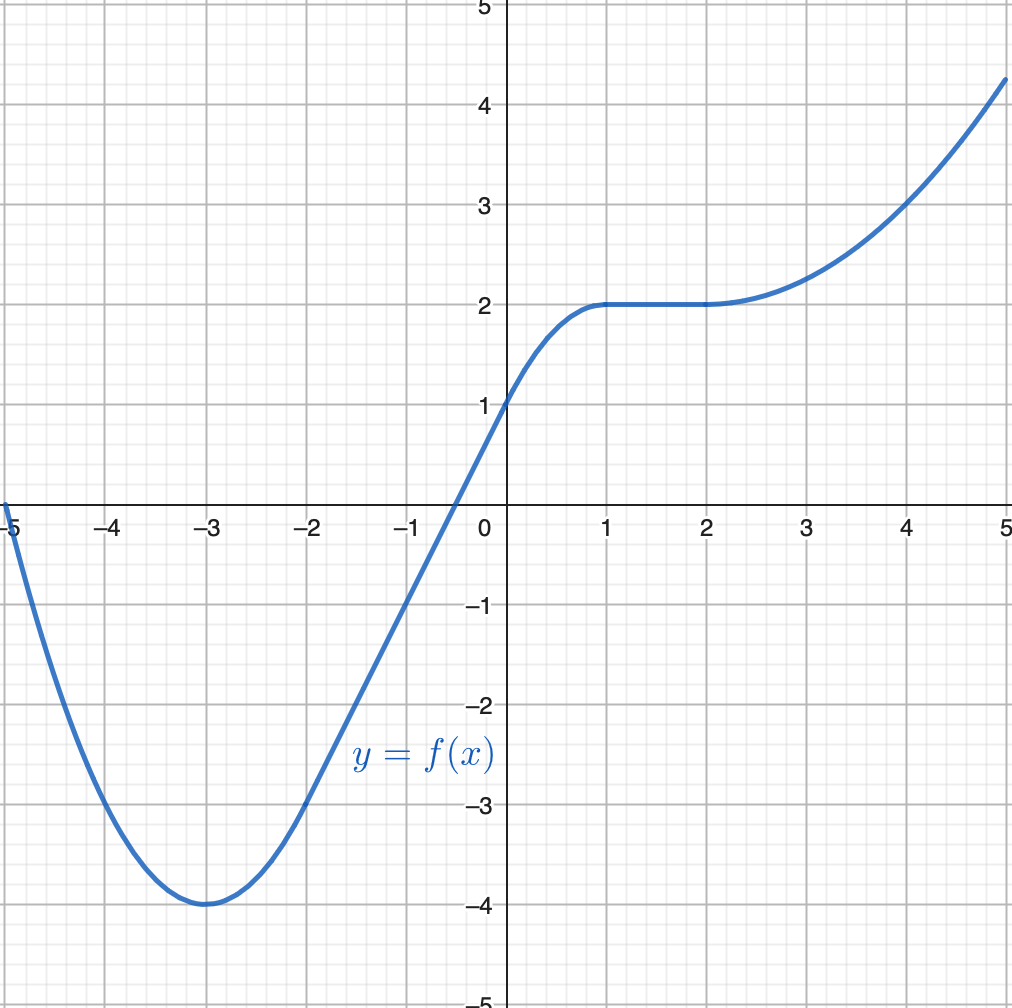
\includegraphics{images/CP-1-LT-1-graph-F23.png}} \hspace{0.25in} \scalebox{0.3}{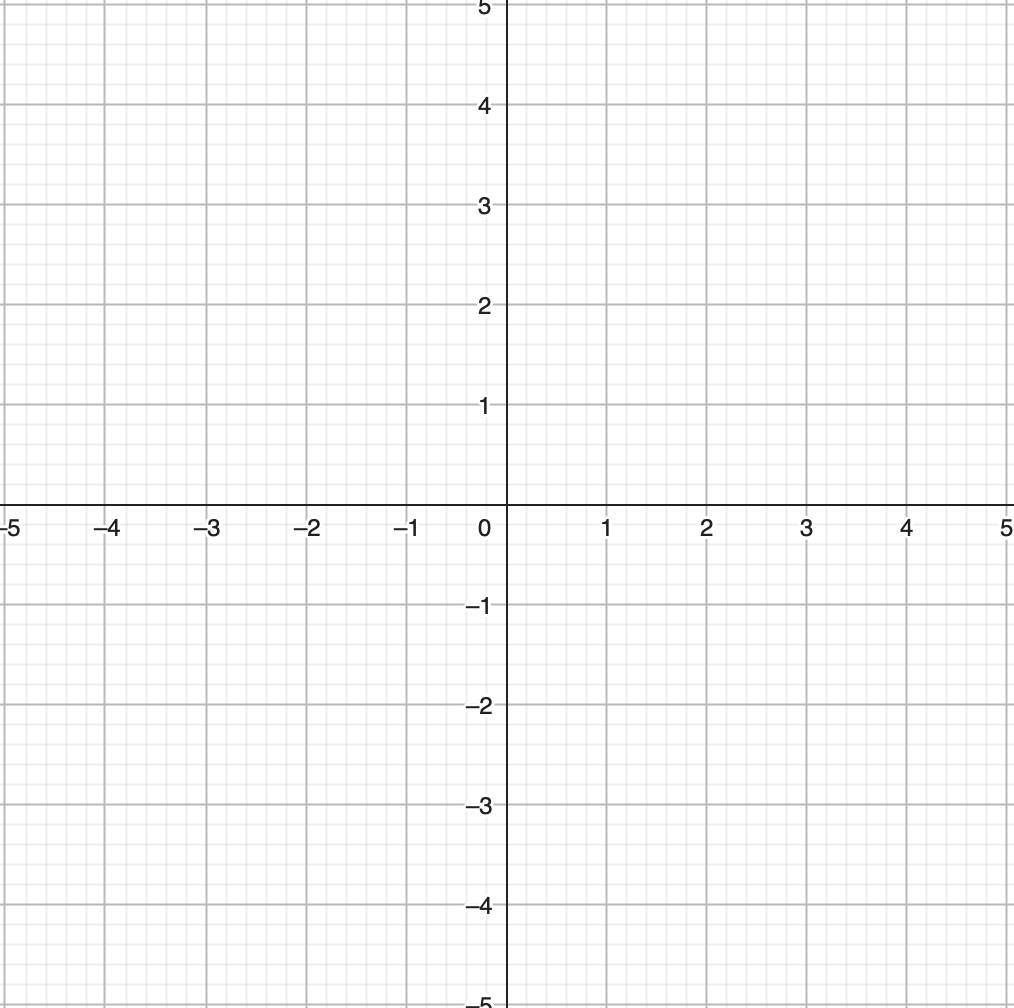
\includegraphics{images/CP-1-LT-1-grid-F23.png}} \\
\end{center}

		\item Consider the two piecewise linear functions $p$ and $q$ given by the figure below.


Determine each of the following derivative values that involve functions that are defined in terms of $p$ and $q$.  Clearly show your work and thinking using proper notation, be sure your values are \emph{exact} in light of the given information.

\begin{center}
\scalebox{0.3}{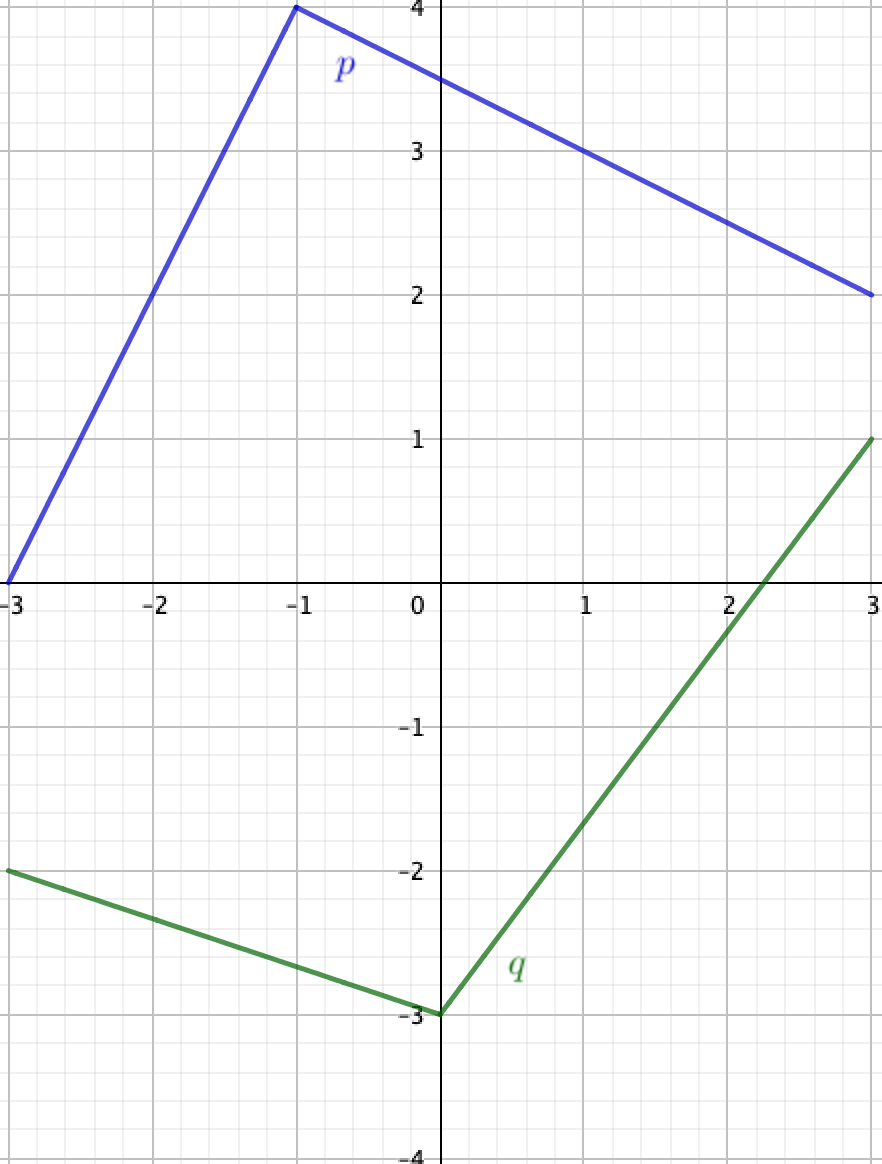
\includegraphics{images/CP7-11-3LTs.png}} \hspace{0.25in} \scalebox{0.5}{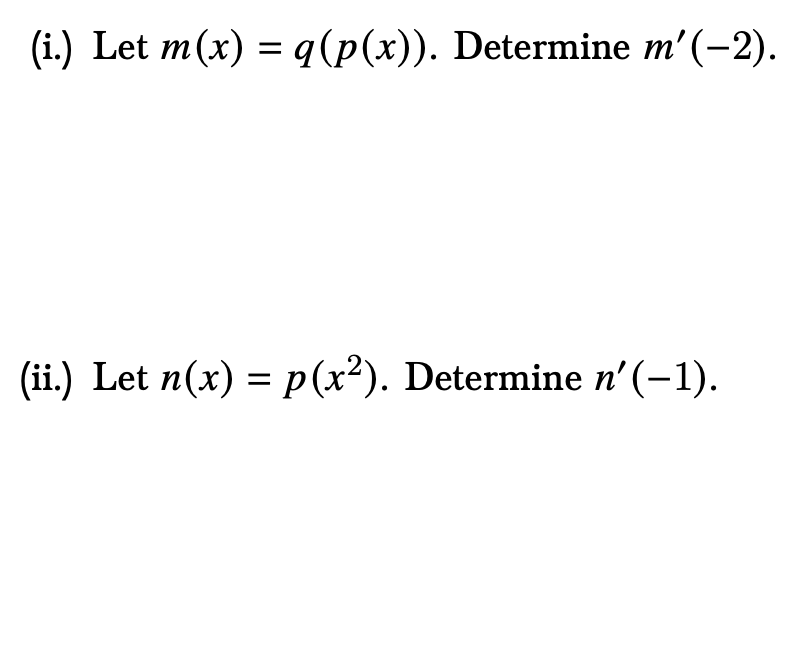
\includegraphics{images/CP-1-side-by-side-F23.png}} 
\end{center}

%\begin{itemize}
%	\item[(i.)] Let $m(x) = q(p(x))$.  Determine $m'(-2)$.
%\lr
%	\item[(ii.)] Let $n(x) = p(x^2)$.  Determine $n'(-1)$.
%	\lr
%\end{itemize}	

		\item Evaluate the following definite integral exactly using the Fundamental Theorem of Calculus.  Show your full work and thinking using proper notation.
		
		$\ds \int_1^3 \left(4x^2 + \frac{1}{x^2} - \frac{2}{x} \right) \, dx$
	\ee
	
	\vfill \hfill {\bf OVER}
	
	\pagebreak
	
	
	\item[2.]  Consider the piecewise linear function $y = g(x)$ pictured below.
	
	\begin{center}
		\scalebox{0.3}{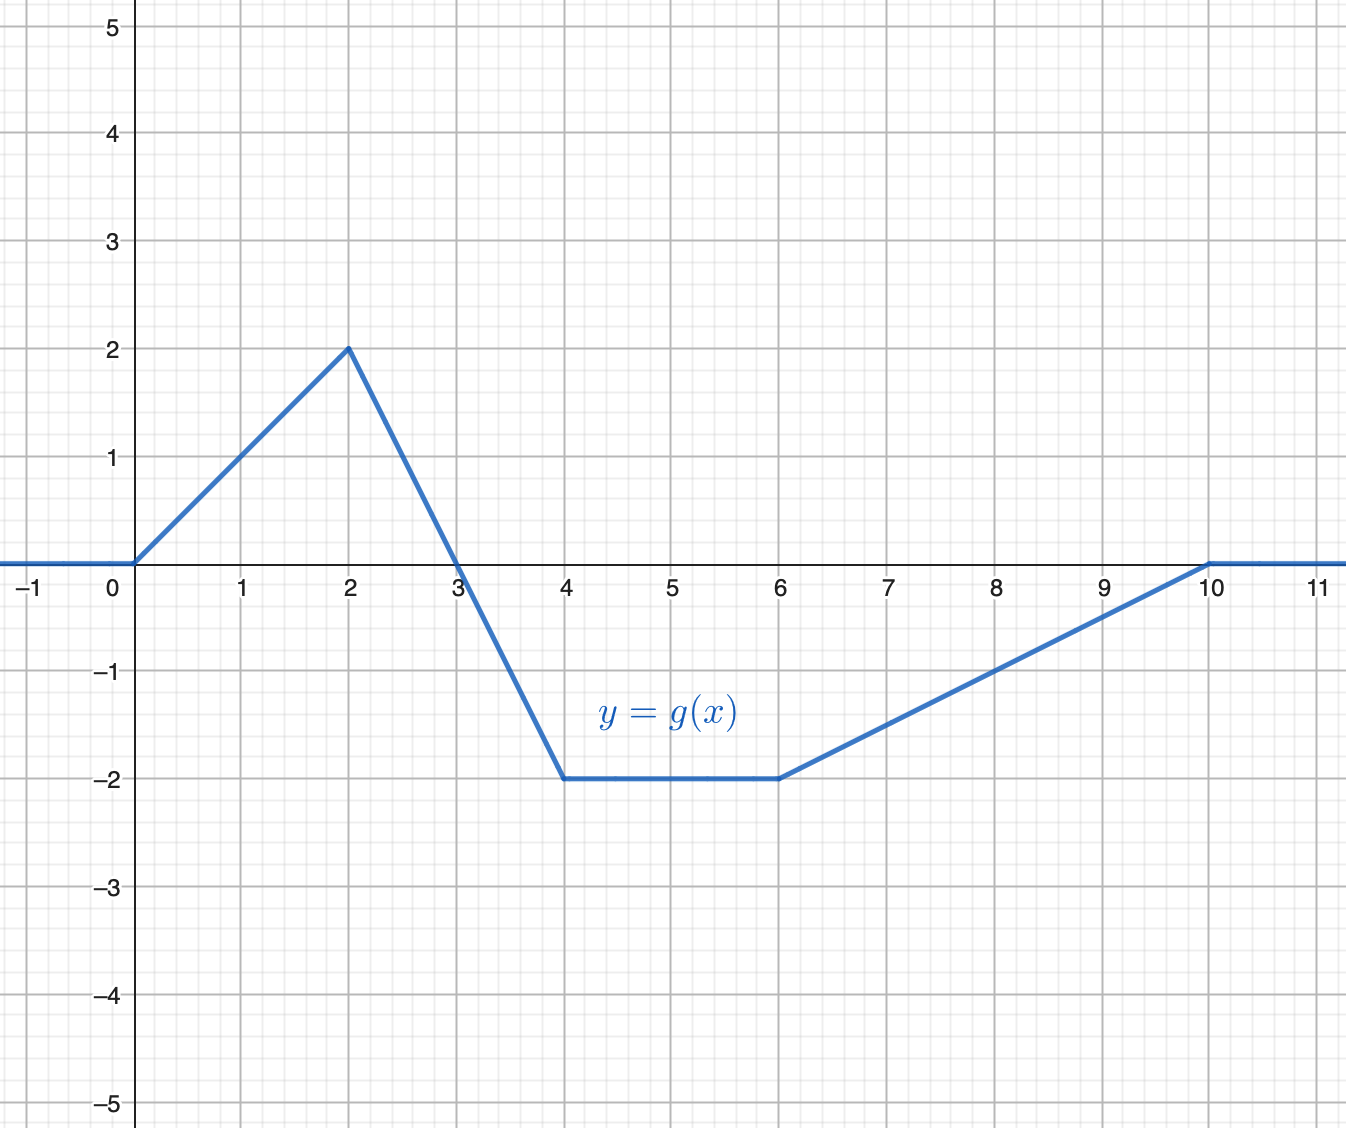
\includegraphics{images/CP-1-LT2-graph-F23.png}} \hspace{0.5in} \scalebox{0.3}{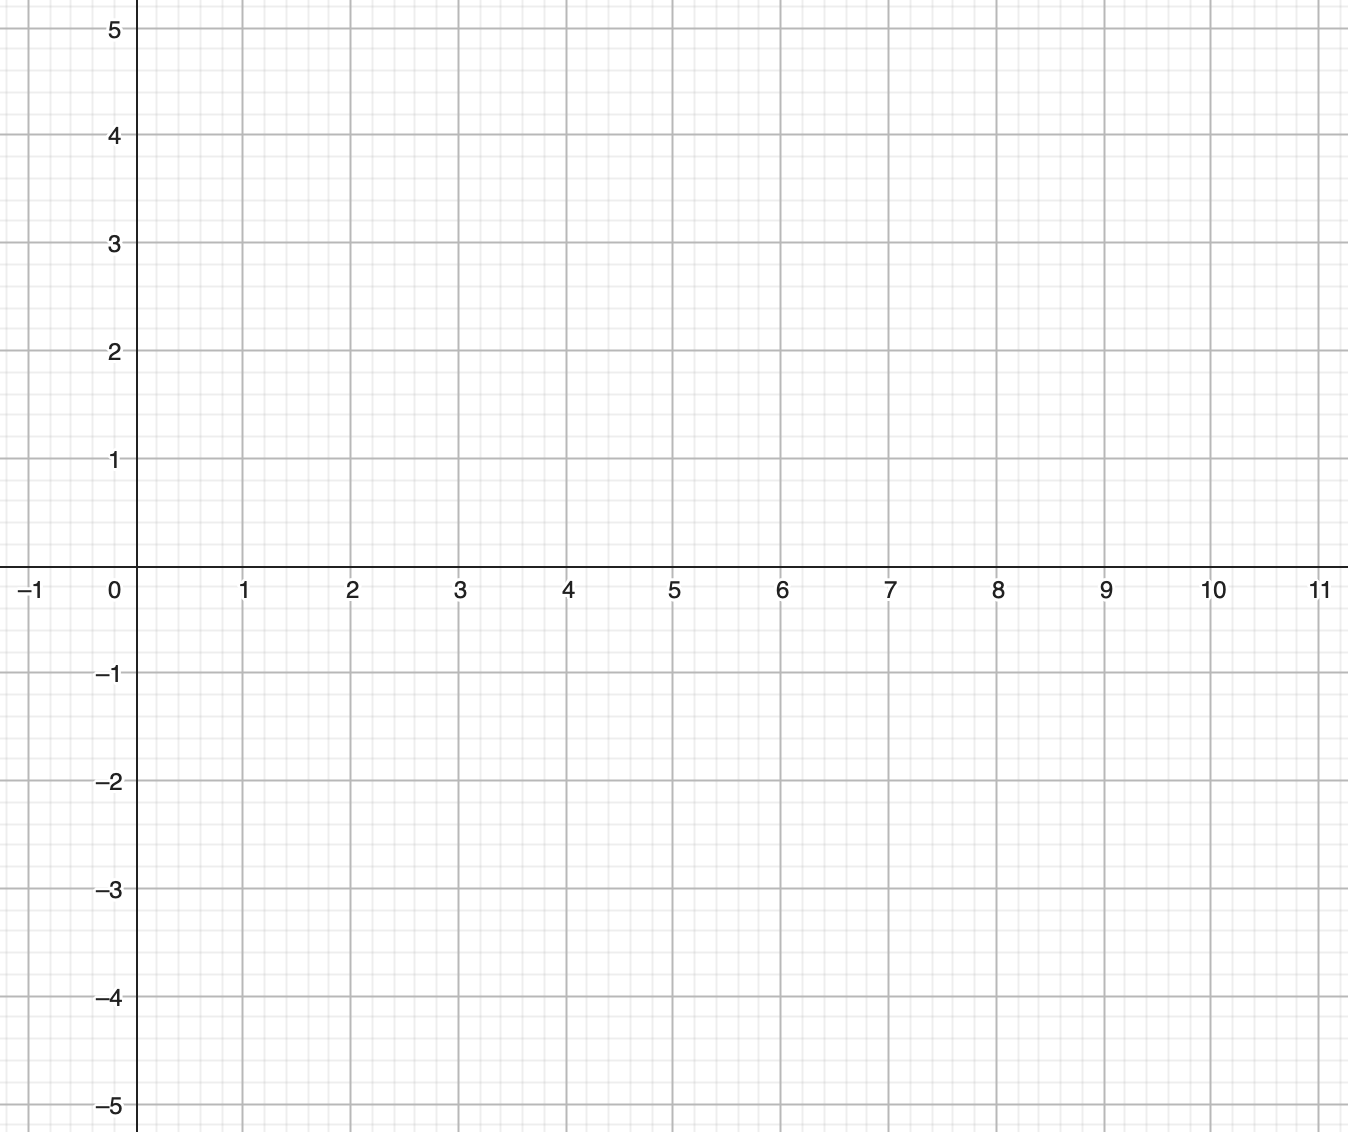
\includegraphics{images/CP-1-LT2-grid-F23.png}} 
	\end{center}
	
	Let $G$ be an antiderivative of $g$ that satisfies $G(0) = 1$.
	
	\be
		\item On what intervals is $G$ increasing?  decreasing? neither?  why?
		
		\lr
		
		\item On what intervals is $G$ concave up?  concave down?  neither?  why?
		
		\lr
		
		\item Find the exact values of $G(2)$, $G(3)$, $G(4)$, $G(6)$, and $G(10)$.  Write one sentence to explain briefly how you found these values.
		
		\mr \tr
		
		\item On the blank grid at right, sketch an accurate, labeled graph of $y = G(x)$.
		
	\ee
\end{enumerate}



\end{document}

